
\documentclass[sigconf]{acmart}

\usepackage{graphicx}
\usepackage{hyperref}
\usepackage{todonotes}

\usepackage{endfloat}
\renewcommand{\efloatseparator}{\mbox{}} % no new page between figures

\usepackage{booktabs} % For formal tables

\settopmatter{printacmref=false} % Removes citation information below abstract
\renewcommand\footnotetextcopyrightpermission[1]{} % removes footnote with conference information in first column
\pagestyle{plain} % removes running headers

\newcommand{\TODO}[1]{\todo[inline]{#1}}

\usepackage{listings}
\usepackage{color}
% \usepackage[parfill]{parskip}

\definecolor{dkgreen}{rgb}{0,0.6,0}
\definecolor{gray}{rgb}{0.5,0.5,0.5}
\definecolor{mauve}{rgb}{0.58,0,0.82}

\lstset{frame=tb,
  language=Python,
  aboveskip=3mm,
  belowskip=3mm,
  showstringspaces=false,
  columns=flexible,
  basicstyle={\small\ttfamily},
  numbers=none,
  numberstyle=\tiny\color{gray},
  keywordstyle=\color{blue},
  commentstyle=\color{dkgreen},
  stringstyle=\color{mauve},
  breaklines=true,
  breakatwhitespace=true
  tabsize=3
}

\def\bZ{\mathbb{Z}}
\def\bN{\mathbb{N}}
\def\bR{\mathbb{R}}
\def\bC{\mathbb{C}}
\def\bQ{\mathbb{Q}}
\usepackage{hyperref}

\usepackage{endfloat}
\renewcommand{\efloatseparator}{\mbox{}} % no new page between figures

\usepackage{booktabs} % For formal tables

\settopmatter{printacmref=false} % Removes citation information below abstract
\renewcommand\footnotetextcopyrightpermission[1]{} % removes footnote with conference information in first column
\pagestyle{plain} % removes running headers
\usepackage{indentfirst}
 
\begin{document}
\title{Diagnosis of Coronary Artery Disease Using Big Data Analysis}


\author{Hady Sylla}
\affiliation{%
  \institution{Indiana University Bloomington}
  \city{Bloomington} 
  \state{Indiana} 
  \postcode{47401}
}
\email{hsylla@iu.edu}



% The default list of authors is too long for headers}
\renewcommand{\shortauthors}{B. Trovato et al.}

 \maketitle
    
\begin{abstract}
    This paper is about Big Data application in the diagnostic of coronary Artery disease .The paper explore contribution that big data had on the analysis of numerous data by researchers.
\end{abstract}
   
    
    \maketitle
\subsection{Introduction}
Cardiovascular illness is the primary source of dreariness and mortality in the Western world\cite{ali}. Early location of coronary corridor ailment (CAD) is of fundamental significance as favorable treatment may permanently lessen grimness and death. Albeit obtrusive coronary angiography remains the standard of reference for the assessment of CAD, multisector processed tomography coronary angiography (CTA) has as of late developed as a reliable imaging methodology for the non-intrusive evaluation of CAD.
THE analysis of coronary-supply route infection on the premise of history and physical examination alone is regularly troublesome. Many complex tests have accordingly been produced to permit an early and more precise analysis. Albeit many tests are presently immovably settled in clinical practice, none is especially suited to wide-scale, savvy application,1 in light of the fact that every ha constraints concerning affectability and specificity. Along these lines, when a positive test outcome happens in a patient with a low probability of illness, it is of restricted analytic importance.2 3 4 A "positive" electrocardiographic anxiety test in an asymptomatic patient, for instance, has a prescient precision of just 30 for every penny for the nearness of angiographic coronary-conduit malady.


\section{Dataset}
For this project  will use Z-Alizadeh Sani aataset for the data analuysis.
    
\section{Analytic}
    I will use Random Forest machine learning for predicting the feature to diagnose coronary artery disease.

\section{Risk factors}
\par In spite of the fact that an extensive variety of hazard factors for coronary heart dis-ease have been distinguished from populace ponders, these measures, separately or in blend, are inadequately pow-erful to give a solid, noninvasive conclusion of the nearness of coronary illness. Here we demonstrate that pat-tern-acknowledgment systems connected to proton atomic mag-netic reverberation (1H-NMR) spectra of human serum can effectively analyze the nearness, as well as the seriousness, of coronary illness. Utilization of super-vised halfway minimum squares-discriminant examination to orthogo-nal flag amended informational collections permits >90% of subjects with stenosis of every one of the three noteworthy coronary vessels to be distin-guished from subjects with angiographically ordinary coro-nary supply routes, with a specificity of >90%. Our examinations appear out of the blue a system fit for giving an accu-rate, noninvasive and fast conclusion of coronary heart dis-facilitate that can be utilized clinically, either in populace screening or to permit compelling focusing of medicines, for example, statins.
Coronary illness (CHD) is a noteworthy reason for mortality and bleakness in created nations, influencing upwards of one of every three people previously the age of 70 years1. In the course of recent decades a scope of ecological and biochemi-cal chance elements for the advancement of CHD have been iden-tified in cross-sectional studies2. For instance, tobacco smoking is related with a roughly two-overlap in-wrinkled danger of CHD3. Additionally, abnormal amounts of cholesterol in substantial, triglyceride-rich lipoprotein particles (mostly low-thickness lipoprotein (VLDL) and low-thickness lipoprotein (LDL)) and lower levels of cholesterol in high-thickness lipoprotein (HDL) particles are known to be related with expanded danger of CHD4.
As of late, be that as it may, there have been specialized advances that have permitted to a great degree high-thickness informational collections to be developed from people. Methods, for example, genomics, proteomics and metabonomics (a frameworks way to deal with ex-amining the adjustments in hundreds or thousands of low-mol-ecular-weight metabolites in an in place tissue or biofluid9) offer the possibility of effectively recognizing people with specific malady or lethal states. Of these methods, NMR-based metabonomics offers a few particular preferences in a clinical setting. To begin with, it can be completed on standard arrangements of serum, plasma or urine10,11, evading the requirement for master arrangements of cell RNA and ace tein required for genomics and proteomics, respectively12– 14. Second, huge numbers of the hazard factors effectively recognized, (for example, levels of different lipids) are little atom metabolites that will add to the metabonomic informational collection.

\section{Analytic}
\begin{lstlisting}
In [2]: import matplotlib.pyplot as plt
    % matplotlib inline
    from sklearn.metrics import accuracy_score

In [4]:from sklearn.ensemble import RandomForestClassifier
        import pandas as pd
        from sklearn.preprocessing import LabelEncoder
        import numpy as np
        df=pd.read_excel('Z-Alizadeh sani dataset.xlsx')
        df.head()
\end{lstlisting}
\includegraphics[width=0.95\columnwidth]

\begin{lstlisting}
In [6]:def extract_col(df,col_name):
        return list(df[col_name])

        col = extract_col(df,'BMI') 
        plt.hist(col)
        plt.show()
\end{lstlisting}
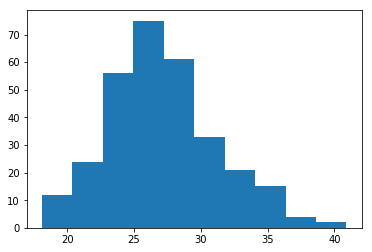
\includegraphics[width=0.95\columnwidth]{project/output_2_0.png}

\begin{lstlisting}
2.1 Taking all categorical features that have only 2 levels and label encoding them to get binary features

In [2]:cols = df.columns
        num_cols = df._get_numeric_data().columns
        cat_cols=list(set(cols) - set(num_cols))
        ##BBB, VHD have multiple levels rest are binary
        ###Cath is predictor var
        cat_cols.remove('VHD')
        cat_cols.remove('Cath')
        cat_cols.remove('BBB')
        cat_cols
\end{lstlisting}

\begin{lstlisting}
Out[2]:['DLP',
    'CRF',
    'Obesity',
    'Poor R Progression',
    'Exertional CP',
    'Airway disease',
    'LowTH Ang',
    'Sex',
    'Nonanginal',
    'Diastolic Murmur',
    'Dyspnea',
    'Thyroid Disease',
   'Lung rales',
    'CVA',
    'CHF',
    'Weak Peripheral Pulse',
    'Atypical',
    'LVH',
    'Systolic Murmur']
\end{lstlisting}

\begin{lstlisting}
In [3]:### Fitting our Encoder
In [4]:df[cat_cols]=df[cat_cols].apply(LabelEncoder()
.fit_transform)
\end{lstlisting}

\begin{lstlisting}
One hot encoding our multiple level features: 'VHD' and 'BBB'
In [5]:from sklearn.feature_extraction import DictVectorizer
        def encode_onehot(df, cols):
        vec = DictVectorizer()
        vec_data = pd.DataFrame(vec.fit_transform(df[cols].to_dict('records')).toarray())
        vec_data.columns = vec.get_feature_names()
         vec_data.index = df.index
    
        df = df.drop(cols, axis=1)
        df = df.join(vec_data)
        return df
        X = encode_onehot(df, cols=['BBB'])
        X1 =encode_onehot(X, cols=['VHD'])
        X1.columns
\end{lstlisting}
\subsubsection{Taking all categorical features that have only 2 levels
and label encoding them to get binary
features}\label{taking-all-categorical-features-that-have-only-2-levels-and-label-encoding-them-to-get-binary-features}
Numerous variable choice strategies depend on the participation of variable significance for positioning and model estimation to create, assess and think about a group of models. Following Kohavi and John (1997) and Guyon and Elisseff (2003), it is common to recognize three sorts of variable determination techniques: "channel" for which the score of variable significance does not rely upon a given model outline strategy; "wrapper" which incorporate the expectation execution in the score figuring; lastly "implanted" which join all the more firmly factor choice and model estimation \cite{GENUER20102225}.
\includegraphics[width=0.95\columnwidth]

\begin{lstlisting}

Out[5]: 
Index(['Age', 'Weight', 'Length', 'Sex', 'BMI', 'DM', 'HTN', 'Current Smoker',
       'EX-Smoker', 'FH', 'Obesity', 'CRF', 'CVA', 'Airway disease',
       'Thyroid Disease', 'CHF', 'DLP', 'BP', 'PR', 'Edema',
       'Weak Peripheral Pulse', 'Lung rales', 'Systolic Murmur',
       'Diastolic Murmur', 'Typical Chest Pain', 'Dyspnea', 'Function Class',
       'Atypical', 'Nonanginal', 'Exertional CP', 'LowTH Ang', 'Q Wave',
       'St Elevation', 'St Depression', 'Tinversion', 'LVH',
       'Poor R Progression', 'FBS', 'CR', 'TG', 'LDL', 'HDL', 'BUN', 'ESR',
       'HB', 'K', 'Na', 'WBC', 'Lymph', 'Neut', 'PLT', 'EF-TTE', 'Region RWMA',
       'Cath', 'BBB=LBBB', 'BBB=N', 'BBB=RBBB', 'VHD=Moderate', 'VHD=N',
       'VHD=Severe', 'VHD=mild'],
        dtype='object')
\end{lstlisting}

\begin{lstlisting}
Getting our pred variable and removing from orignal df
In [6]:y=df["Cath"].map({'Cad':0,'Normal':1})
    X1.drop('Cath',1,inplace=True)
\end{lstlisting}
\begin{lstlisting}
Splitting into train and test
In [8]:from sklearn.model_selection import train_test_split
    X_train, X_test, y_train, y_test = train_test_split(X1, y, test_size=0.2, random_state=3)
\end{lstlisting}
\begin{lstlisting}
Hypertuning our featureset using grid search to get best possible params
In [21]:from sklearn.model_selection import GridSearchCV
    Depth=[2,3,4,5]
    Trees=[200,500,700]
    tuned_parameters = [{'n_estimators': Trees,'max_depth':Depth}]              
    RFM = RandomForestClassifier()
    clf = GridSearchCV(RFM, tuned_parameters, cv=5,scoring='accuracy')
    clf.fit(X1,y)
    print("Best parameters set found on development set:")
    print()
    print(clf.best_params_)
\end{lstlisting}
\begin{lstlisting}

Best parameters set found on development set:

{'max_depth': 5, 'n_estimators': 200}
In [22]:scores = [x[1] for x in clf.grid_scores_]
    scores = np.array(scores).reshape(len(Depth), len(Trees))
    for ind, i in enumerate(Depth):
    plt.plot(Trees, scores[ind], label='max_depth: ' + str(i))
    plt.legend()
    plt.xlabel('n_estimators')
    plt.ylabel('Mean score')
    plt.show()
`
\end{lstlisting}
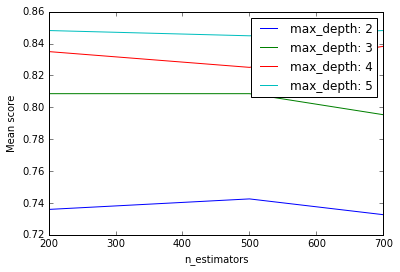
\includegraphics[width=0.95\columnwidth]{project/output_15_1.png}

\begin{lstlisting}

This is for plotting our feature importances with their standard deviations
In [23]:clfs = RandomForestClassifier(n_estimators= clf.best_params_['n_estimators'],
max_depth=clf.best_params_['max_depth'])
    clfs.fit(X1, y.ravel())

    importance = clfs.feature_importances_
    importance = pd.DataFrame(importance, index=X1.columns, 
    columns=["Importance"])

    importance["Std"] = np.std([tree.feature_importances_
    for tree in clfs.estimators_], axis=0)

    x = range(importance.shape[0])
    y = importance.ix[:, 0]
    yerr = importance.ix[:, 1]

    plt.bar(x, y, yerr=yerr, align="center")

    plt.show()
\end{lstlisting}
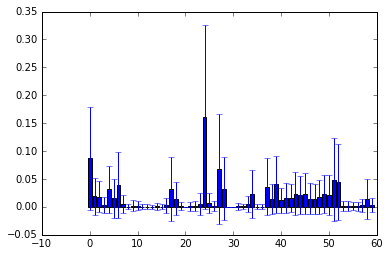
\includegraphics[width=0.95\columnwidth]{project/output_17_0.png}

\begin{lstlisting}
In [24]:importance
\end{lstlisting}

\includegraphics[width=0.95\columnwidth]

\includegraphics[width=0.95\columnwidth]
\begin{lstlisting}
Importance	Std
\end{lstlisting}


This table show the importance of each feature in the diagnostic of CAD. Based on the analysis the age, HTN,  DM, BP, Typical chest pain, Non-Anginal  CP, T  inversion, Q  wave,  ST elevation, PR, and ST depression are the features with the highest impact on CAD.

Variable significance is figured restrictively to a given acknowledgment notwithstanding for reproduced datasets. This decision which is criticizable if the goal is to achieve a decent estimation of a basic steady, is predictable with remaining as near as conceivable to the exploratory circumstance managing a given dataset\cite{GENUER20102225}.
\includegraphics[width=0.95\columnwidth]

\begin{lstlisting}

Out[24]:
Age	0.086779	0.092552
Weight	0.018672	0.032956
Length	0.018183	0.027928
Sex	0.003414	0.013603
BMI	0.031609	0.042215
DM	0.015427	0.034442
HTN	0.038735	0.059296
Current Smoker	0.005287	0.015965
EX-Smoker	0.000587	0.004463
FH	0.002472	0.010216
Obesity	0.002333	0.008439
CRF	0.000534	0.004805
CVA	0.000469	0.004108
Airway disease	0.000474	0.003385
Thyroid Disease	0.001086	0.006045
CHF	0.000407	0.004046
DLP	0.003296	0.013382
BP	0.031988	0.056958
PR	0.014277	0.029568
Edema	0.001758	0.007496
Weak Peripheral Pulse	0.000000	0.000000
Lung rales	0.001332	0.007931
Systolic Murmur	0.001853	0.008916
Diastolic Murmur	0.004950	0.020264
Typical Chest Pain	0.161378	0.165277
Dyspnea	0.006237	0.017810
Function Class	0.001798	0.008412
Atypical	0.067681	0.098911
Nonanginal	0.032299	0.056285
Exertional CP	0.000000	0.000000
LowTH Ang	0.000000	0.000000
Q Wave	0.000976	0.005923
St Elevation	0.000906	0.004613
St Depression	0.005336	0.014798
Tinversion	0.022593	0.042821
LVH	0.000687	0.004452
Poor R Progression	0.000546	0.004018
FBS	0.036382	0.051744
CR	0.014378	0.027248
TG	0.040267	0.051599
LDL	0.011746	0.022602
HDL	0.015883	0.027084
BUN	0.015708	0.025022
ESR	0.023733	0.038713
HB	0.021479	0.033380
K	0.023375	0.036937
Na	0.014249	0.027810
WBC	0.014354	0.026839
Lymph	0.018147	0.030376
Neut	0.022351	0.034163
PLT	0.021242	0.035043
EF-TTE	0.049034	0.074234
Region RWMA	0.044669	0.068886
BBB=LBBB	0.001229	0.008498
BBB=N	0.002322	0.008860
BBB=RBBB	0.000986	0.006953
VHD=Moderate	0.001554	0.008084
VHD=N	0.002828	0.011718
VHD=Severe	0.014135	0.036448
VHD=mild	0.003587	0.013188

\end{lstlisting}

\begin{lstlisting}
\large Final checking of our model's accuracy on test set
In [25]:
clf = RandomForestClassifier(n_estimators= clf.best_params_['n_estimators'],max_depth=clf.best_params_['max_depth'])
clf.fit(X_train, y_train)
y_pred=clf.predict(X_test)
print(accuracy_score(y_test,y_pred))
print()
print()
print('The accuracy score on test by Random Forest:{}'.format(accuracy_score(y_test,y_pred)))
0.885245901639


The accuracy score on test by Random Forest:0.8852459016393442
\end{lstlisting}





   \maketitle
    \subsection{Conclusion}

A period of open data in social insurance is currently under way. We have effectively encountered a time of advance in digitizing therapeutic records, as pharmaceutical organizations and different associations total a long time of innovative work information in electronic databases. The national government and other open partners have additionally quickened the push toward straightforwardness by making many years of put away information usable, accessible, and significant by the medicinal services segment in general. Together, these increments in information liquidity have conveyed the business to the tipping point.



\maketitle
\subsection{Acknowlement}

  I would like to thank Dr. Gregor von Laszewski for his
  support and suggestions to write this paper.




    
    
    


    % Add a bibliography block to the postdoc
    \bibliographystyle{acm}
    \bibliography{report}
    
    \end{document}
